\chapter{Calibración final con IRAF}
En esta última clase revisaremos el procedimiento para calibrar las imágenes de objeto usando IRAF. Esto constituye la calibración básica y posteriormente es posible realizar cualquier tipo de análisis con las imágenes, ya sea análisis fotométrico o espectroscópico. 

\section{Calibración de imágenes}
El paso final de la calibración o reducción básica consiste en utilizar los archivos de master bias y master flat para corregir las imágenes de objeto. Recuerda que los datos de OSIRIS no necesitan ser corregidos por corriente oscura y por lo tanto no necesitamos de un master dark. 

Comenzamos lanzando la interfaz de pyraf desde la terminal para luego movernos a la carpeta donde están nuestros datos:

\begin{shell}
$ pyraf
--> cd OB0001/
-->
\end{shell}

\subsection{Imágenes de objeto}
Las imágenes de interés se encuentran dentro del directorio \pynorm{'object'}. Podemos movernos a esa carpeta y verificar su contenido. 

\begin{shell}
--> pwd
/home/user/OB0001
--> cd object
--> ls
\end{shell}

La carpeta \pynorm{'object'} contiene 47 imágenes en total. El nombre de cada imagen está compuesto de un número o ID, seguido de la fecha y el instrumento. Para visualizarlas, usamos el software \norbash{ds9} que instalamos anteriormente. Por ejemplo, con el siguiente comando se visualiza una de las imágenes de objeto, específicamente la tercera de la carpeta:

\begin{shell}
--> !ds9 0002611439-20200712-OSIRIS-OsirisBroadBandImage1.fits
\end{shell}

\begin{figure}[htb]
  \centering
	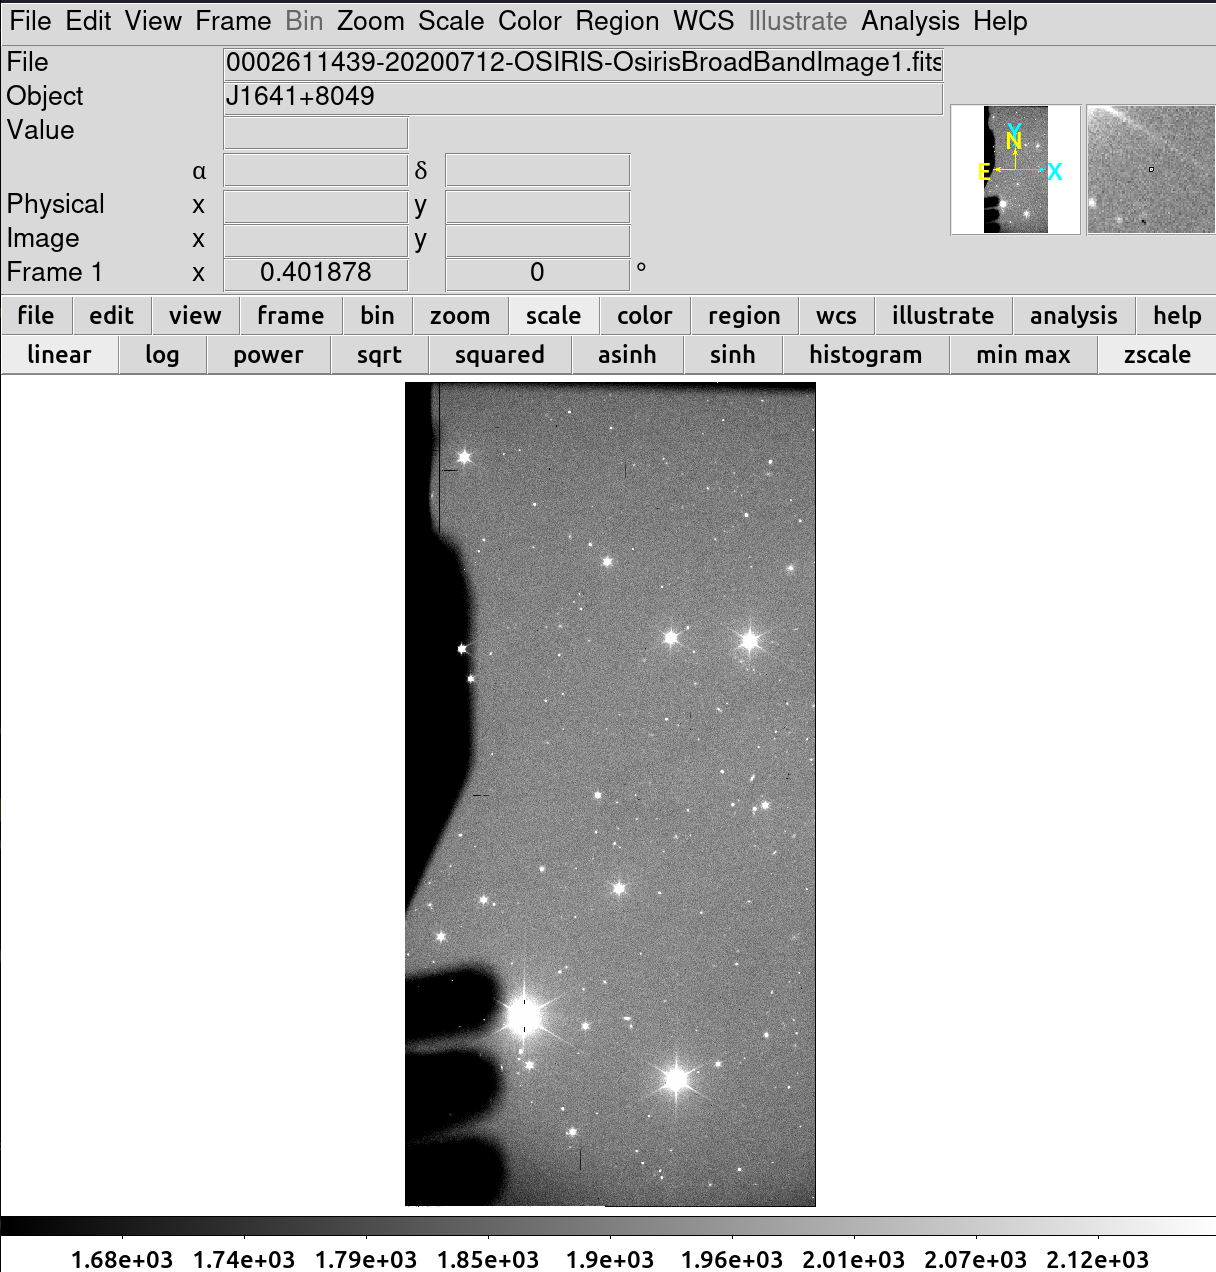
\includegraphics[width=0.7\textwidth]{figures/ds9-campo-completo.png}
	\caption{Imagen de campo completo del instrumento OSIRIS en la ubicación de la viuda negra}
	\label{fig:ds9-campo-completo} 
\end{figure}

Para que obtengas el mismo resultado mostrado en la Figura \ref{fig:ds9-campo-completo}, debes presionar el botón llamado \norbash{scale} y luego \norbash{zscale}. Esto es equivalente a usar la función \norbash{show_image()} en Python. Recuerda que debido a la cantidad de píxeles de estas imágenes, es necesario aplicar una escalación. 

Lo mostrado en la Figura \ref{fig:ds9-campo-completo} corresponde al campo completo de la imagen. Es decir, toda la región detectada por el instrumento. En realidad, es solamente una de las dos regiones detectadas, pero es la única que nos interesa ya que ahí está nuestra viuda negra. Las sombras que aparecen es la rueda de filtros y esa región no se puede usar para el análisis. Esta imagen cuenta con los ruidos de bias y flat, que se hace más evidente si abrimos otra de las imágenes. 

Si cerramos \norbash{ds9} y ejecutamos el siguiente comando abriremos otra imagen donde podremos visualizar de mejor manera el ruido:

\begin{shell}
--> !ds9 0002611450-20200712-OSIRIS-OsirisBroadBandImage1.fits
\end{shell}

\begin{figure}[htb]
  \centering
	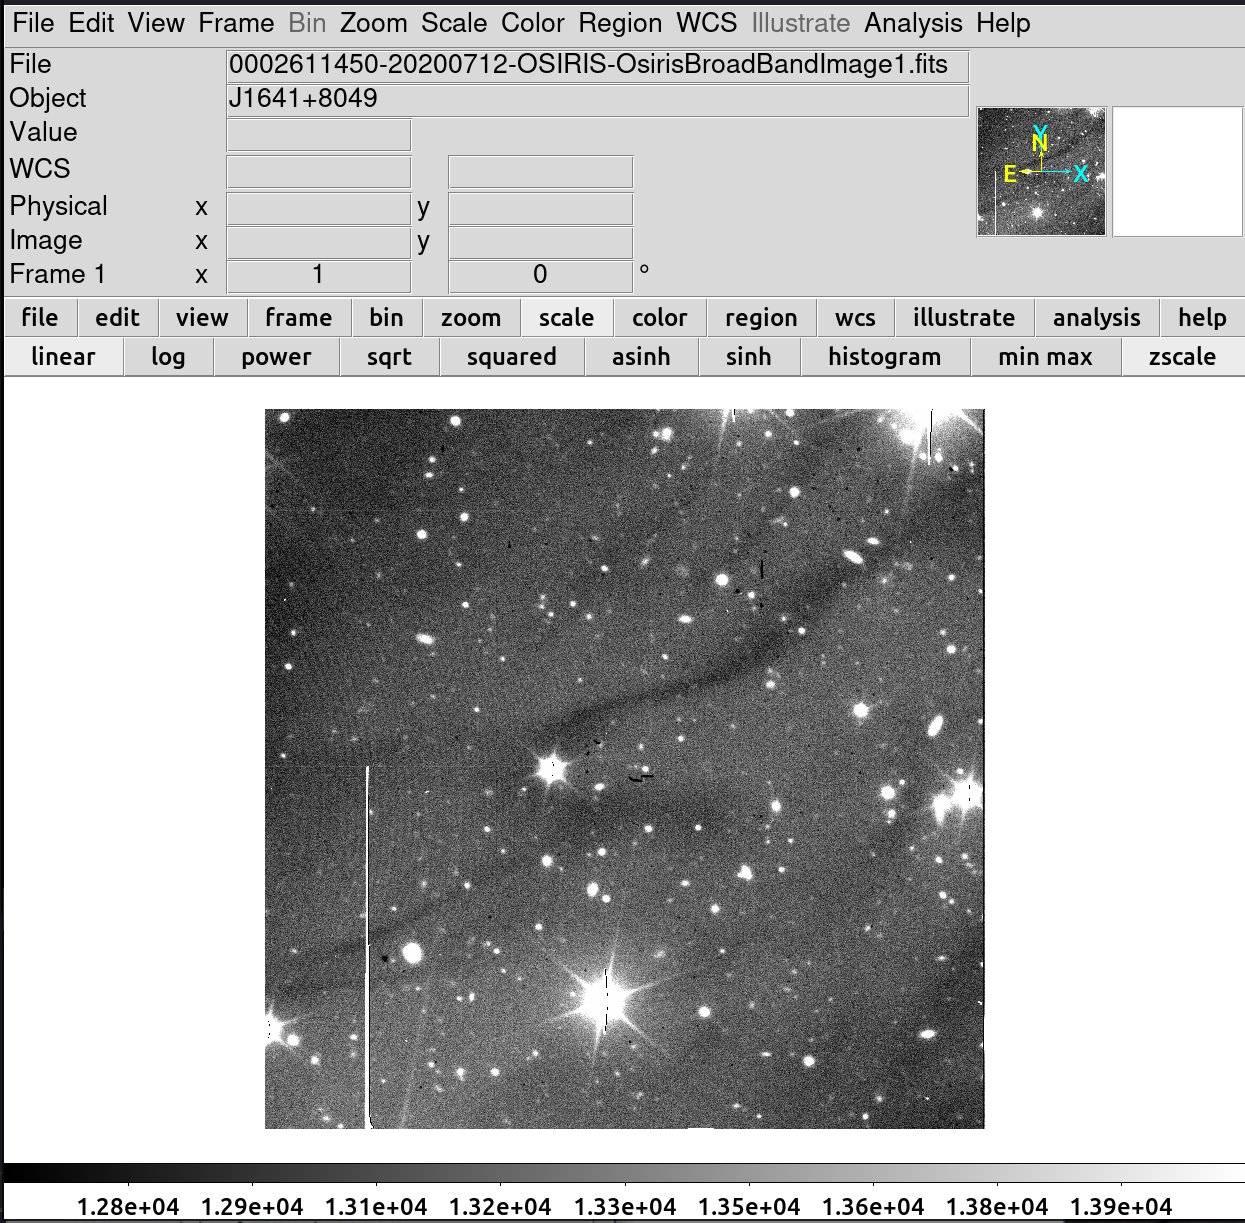
\includegraphics[width=0.7\textwidth]{figures/ds9-noisses.png}
	\caption{Imagen del objeto de interés}
	\label{fig:ds9-noisses} 
\end{figure}

En la Figura \ref{fig:ds9-noisses} se hace evidente la presencia de ondas a lo largo de la imagen. Esas ondas corresponden a la uniformidad en la sensibilidad de los CCD y por lo tanto se trata de ruido debido a los flat fields. Además, esta imagen es más pequeña que la que abrimos anteriormente. Esto se hace a propósito para ahorrar tiempo en la lectura de los CCDs al momento de realizar el análisis y aprovechar los tiempos de observación. 

Como vimos anterormente, en la carpeta \pynorm{'object'} hay 47 imágenes. Tenemos esta gran cantidad de imágenes de objeto porque vamos a analizar datos de una viuda negra. Este tipo de sistemas se caracteriza porque cambia su brillo de manera periódica y para lograr visualizarlo necesitamos una gran cantidad de datos en diferentes ventanas de tiempo. Sin embargo, para realizar la calibración de estos datos, no necesitamos las imágenes de campo completo ni tampoco las que tienen tiempos de exposición corto. Por facilidad, podemos eliminar las primeras 4 imágenes de la carpeta (de la imagen 0002611437 a la 0002611440). O si lo prefieres, solo muévelas a otra carpeta distinta. 

Para ser claros, la carpeta object debe quedar tan solo con 43 imágenes iniciando a partir del elemento con ID 0002611441:
\begin{shell}
--> ls
0002611441-20200712-OSIRIS-OsirisBroadBandImage1.fits
0002611442-20200712-OSIRIS-OsirisBroadBandImage1.fits
0002611443-20200712-OSIRIS-OsirisBroadBandImage1.fits
0002611444-20200712-OSIRIS-OsirisBroadBandImage1.fits
0002611445-20200712-OSIRIS-OsirisBroadBandImage1.fits
...

\end{shell}

Con estas imágenes podemos continuar con el análisis. Primero, debemos crear una lista que contenga los nombres de todos los archivos de imágens de objeto:

\begin{shell}
--> ls *.fits > lista_objeto
-->
\end{shell}

Esta será nuestra lista de entrada, pero al igual que con las imágenes de flat, necesitamos crear una segunda lista para los archivos de salida. Vamos a proceder de la misma manera: editar el archivo de texto llamado \pynorm{'lista_objeto'}, agregar a cada elemento la palabra \pynorm{'corrected'} antes de la extensión \norbash{.fits} y guardarlo como un nuevo archivo dentro de la misma carpeta, al que llamaremos \pynorm{'lista_objeto_corrected'}. Es decir, en nuestra carpeta de objeto deberían haber dos listas distintas: una llamada \pynorm{'lista_objeto'} y otra llamada \pynorm{'lista_objeto_corrected'}. 

Los elementos de la lista \pynorm{'lista_objeto'} deberían verse así:
\begin{shell}
--> tail lista_objeto
0002611478-20200712-OSIRIS-OsirisBroadBandImage1.fits
0002611479-20200712-OSIRIS-OsirisBroadBandImage1.fits
0002611480-20200712-OSIRIS-OsirisBroadBandImage1.fits
0002611481-20200712-OSIRIS-OsirisBroadBandImage1.fits
0002611482-20200712-OSIRIS-OsirisBroadBandImage1.fits
0002611483-20200712-OSIRIS-OsirisBroadBandImage1.fits

\end{shell}

Mientras que los elementos de la lista \pynorm{'lista_objeto_corrected'} deberían verse así:

\begin{shell}
--> tail lista_objeto_corrected
0002611478-20200712-OSIRIS-OsirisBroadBandImage1_corrected.fits
0002611479-20200712-OSIRIS-OsirisBroadBandImage1_corrected.fits
0002611480-20200712-OSIRIS-OsirisBroadBandImage1_corrected.fits
0002611481-20200712-OSIRIS-OsirisBroadBandImage1_corrected.fits
0002611482-20200712-OSIRIS-OsirisBroadBandImage1_corrected.fits
0002611483-20200712-OSIRIS-OsirisBroadBandImage1_corrected.fits
\end{shell}

Antes de aplicar la corrección, debemos elimiar los headers llamados \pynorm{'DATASEC'} y \pynorm{'CCDSEC'} de la misma forma que lo hicimos en la clase anterior. En esta ocasión debemos colocar como entrada a la lista llamada \pynorm{'lista_objeto'} y ejecutar:

\begin{shell}
--> epar hedit
\end{shell}

\begin{figure}[htb]
  \centering
	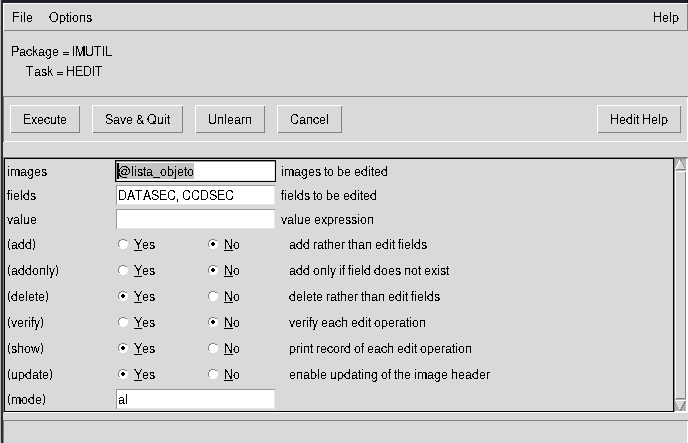
\includegraphics[width=\textwidth]{figures/pyraf-hedit-objeto.png}
	\caption{Parámetros para eliminar headers de las imágenes de objeto.}
	\label{fig:pyraf-hedit-objeto} 
\end{figure}

Cuando el proceso termine, podemos corregir las imágenes de objeto por bias y por flat. Para eso utilizamos otra vez la tarea \norbash{ccdproc}. La lista de entrada es \pynorm{'lista_objecto'}, la lista de salida es \pynorm{'lista_objeto_corrected'}, el parámetro \pynorm{'ccdtype'} debe quedar vacío. Además, en esta ocasión seleccionaremos el campo \pynorm{'Apply zero level correction?'} y \pynorm{'Apply flat field correction?'} en \norbash{Yes} y todo lo demás en \norbash{No}. Finalmente, debemos especificar la ruta hacia el master bias y el master flat en los campos correspondientes. Si tienes alguna duda, revisa la Figura \ref{fig:pyraf-object-correction}.

\begin{shell}
--> epar ccdproc
\end{shell} 

\begin{figure}[htb]
  \centering
	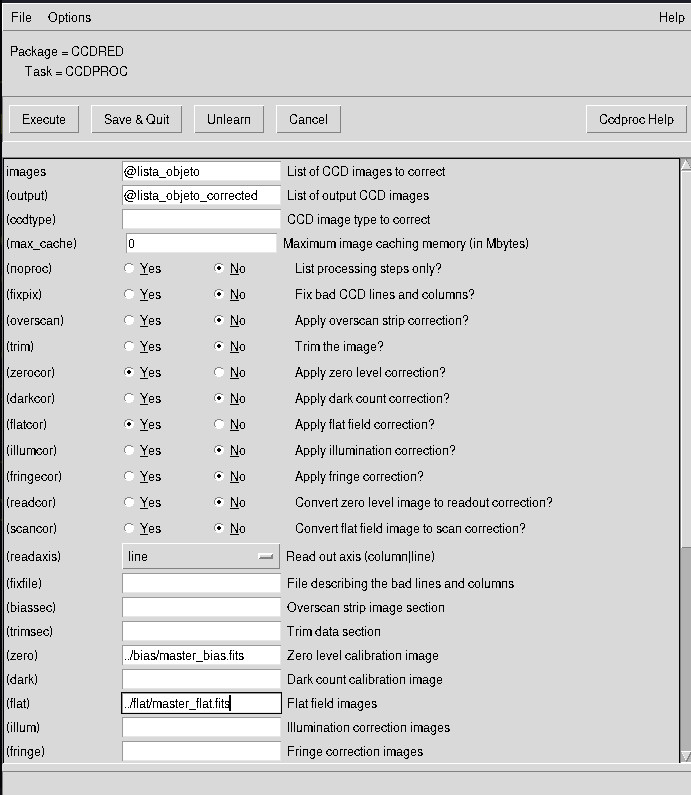
\includegraphics[width=0.7\textwidth]{figures/pyraf-object-correction.png}
	\caption{Parámetros para corregir las imágenes de objeto con \norbash{ccdproc}.}
	\label{fig:pyraf-object-correction} 
\end{figure}

Esta tarea puede tomar bstantes segundos o minutos dependiendo de tu computadora. Cuando termine, puedes revisar el resultado de cualquiera de las imágenes generadas usando de nuevo \norbash{ds9}. Por ejemplo, podemos visualizar la misma imagen que abrimos anteriormente, pero ya corregida. Dicha imagen es la que tiene el ID 0002611450.

\begin{shell}
--> !ds9 0002611450-20200712-OSIRIS-OsirisBroadBandImage1_corrected.fits
\end{shell}

El resultado se muestra en la Figura \ref{fig:object-corrected}. En esta imagen ya no aparecen las ondas debidas a los ruidos de flat field, tampoco aparecen los ruidos debido al bias. Nuevamente, recuerda que justo en eso consiste la reducción básica: corregir las imágenes por cualquier fuente de ruido debida al instrumento.

Con esta lista de imágenes podemos intentar realizar un análisis fotométrico bastante simple. El primer paso consiste en alinear las imágenes para que la estrella de interés aparezca siempre en la misma posición. En este documento se explica cómo alinear una sola imagen, tu tarea es alinear todas las demás. 

\begin{figure}[htb]
  \centering
	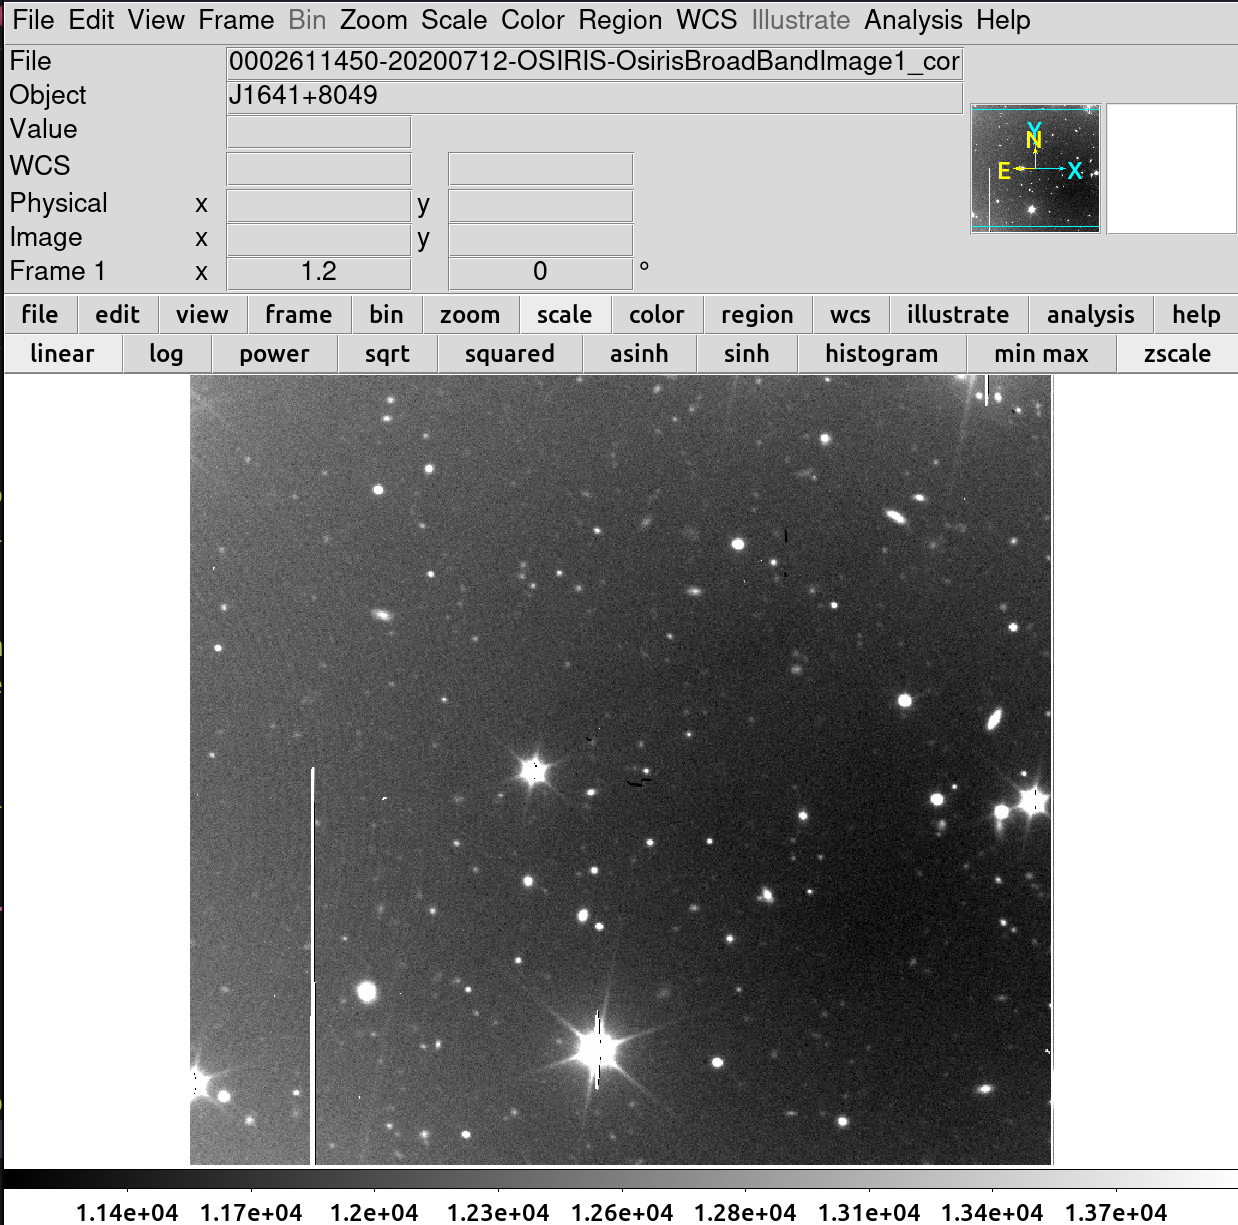
\includegraphics[width=0.7\textwidth]{figures/ds9-object-corrected.png}
	\caption{Imagen de objeto corregida por bias y por flat.}
	\label{fig:object-corrected} 
\end{figure}

Primero abre todas las imágenes corregidas del objeto al mismo tiempo usando \norbash{ds9}, por ejemplo con el comando

\begin{shell}
--> !ds9 *_corrected.fits
\end{shell}

Cuando \norbash{ds9} termine de cargar todas las imágenes, da clic sobre cualquiera de ellas. Luego dirígete al apartado llamado <<\norbash{Frame}>> en la barra de menú de la parte superior de \norbash{ds9} y da clic en: \bashbold{Frame -> Single Frame}. Ahora para visualizar mejor la imagen presiona el botón \bashbold{scale} y luego el de \bashbold{zscale}. Posteriormente, dirígete nuevamente a la barra de menú y da clic en \bashbold{Frame -> Match -> Frame -> Image}. Una vez que lo hagas, repite para \bashbold{Frame -> Match -> Scale}. Si ahora presionas la tecla \norbash{Tab}, te moveras a la siguiente imagen que ya tiene aplicada la misma escala. Presiona \norbash{Tab} una y otra vez y notarás que las imágenes no están alineadas. El mismo objeto encada imagen parece desplazarse como en las esquinas de un cuadrado, de modo que cada cuatro imágenes regresa a su posición inicial. El objeto que nos interesa se muestra en la Figura \ref{fig:ds9-viuda-negra}, justo al centro de la imagen.

\begin{figure}[htb]
  \centering
				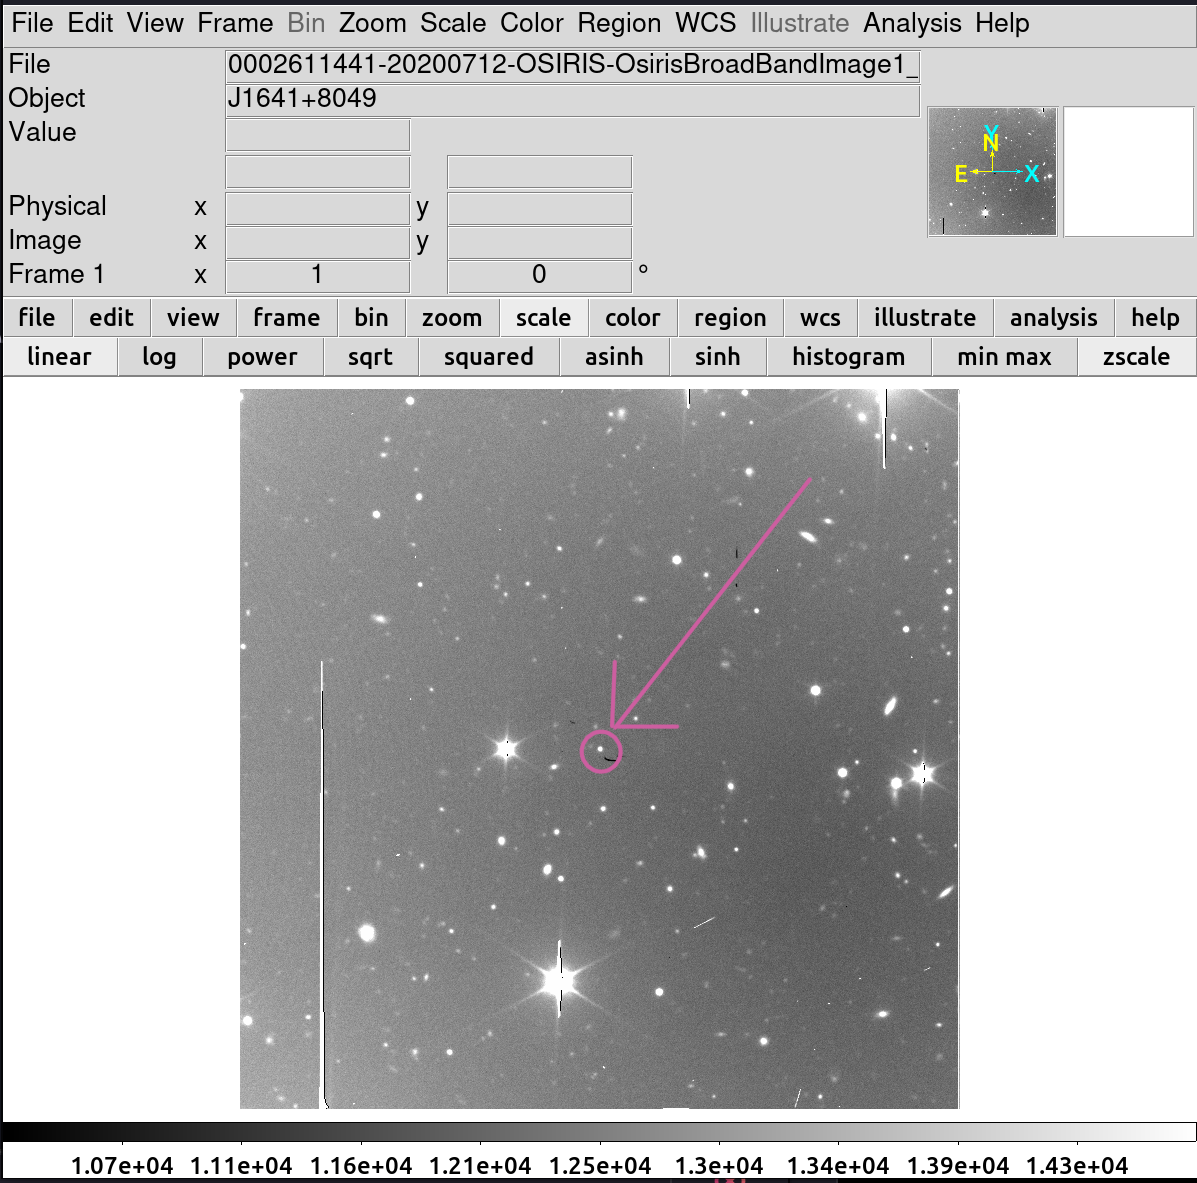
\includegraphics[width=0.7\textwidth]{figures/ds9-viuda-negra.png}
				\caption{Ubicación de la viuda negra en los datos}
				\label{fig:ds9-viuda-negra} 
\end{figure}

Al ubicar el puntero sobre la viuda negra en la imagen 0002611441, parece que se ubica aproximadamente en el píxel 360 en el eje $ x $ y en el píxel 360 en el eje $ y $. Si repites este procedimiento para la imagen 0002611442, ahora la viuda negra se ubica en los pixeles 380 y 360 sobre el eje $ x $ y eje $ y $, respectivamente. Es decir, se desplazó 20 píxeles a la derecha. Si repetimos para la imagen 0002611443, la viuda negra se ubica en los píxeles 380 y 340 sobre el eje $ x $ y eje $ y $, respectivamente. Es decir, ahora está desplazada 20 píxeles hacia abajo y 20 a la derecha con respecto a la imagen inicial. Si seguimos así nos daremos cuenta que la imagen 0002611444 está desplazada 20 pixeles hacia abajo de la imagen inicial, sin desplazamiento horizontal. Finalmente, la imagen 0002611445 vuelve a estar en la misma posición que la imagen inicial y todo esto se repite en las siguientes imágenes.

La tarea es simple: hacer que todas las imágenes tengan a la viuda negra en la misma ubicación. Esto lo logramos con la herramienta llamada \norbash{imshift} de IRAF/Pyraf. Para usarla, como es costumbre, ejecutamos el comando \norbash{epar imshift}.

\begin{shell}
--> epar imshift
\end{shell}
La interfaz de esta herramienta se muestra en la Figura \ref{fig:pyraf-imshift}. En este ejemplo se desplazará a la imagen 0002611442 20 píxeles a la izquierda, para que regrese a la ubicación de la imagen 0002611441. 

\begin{figure}[htb]
  \centering
				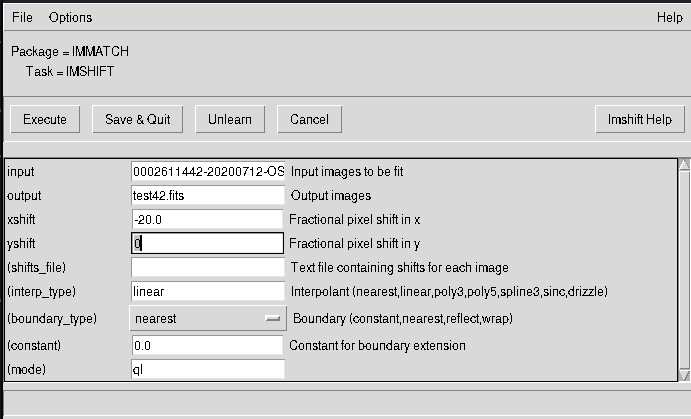
\includegraphics[width=0.7\textwidth]{figures/pyraf-imshift-42.png}
				\caption{Parámetros para desplazar pixeles en las imágenes usando \norbash{imshift}.}
				\label{fig:pyraf-imshift} 
\end{figure}

Al presionar el botón de \bashbold{Ejecutar} se creará una imagen llamada \pynorm{'test42.fits'} que estará desplazada 20 píxeles a la izquierda. Este procedimeinto se debe repetir para todas las demás imágenes teniendo cuidado de cuáles se desplazan a la izquierda, cuáles hacia arriba y cuáles en una combinación de ambas direcciones. Por ejemplo, por el análisis descrito anteiormente, sabemos que la imagen 0002611443 debe desplazarse 20 píxeles a la izquierda (\pynorm{-20} en $ x $ en \norbash{imshift}) y 20 píxeles hacia arriba (\pynorm{20} en $ y $ en \norbash{imshift}). La imagen 0002611444 debe desplazarse 20 píxeles hacia arriba (\pynorm{20} en $ y $ en \norbash{imshift}) y la imagen 0002611445 no debe desplazarse ningún píxel. Además de repetir el ciclo para todas las demás imágenes. 

\subsection{Ejercicios}
Repite el procedimiento de alineación de imágenes para todas las imágenes de objeto calibradas restantes. Puedes hacerlo una por una o crear listas de imágenes que se moverán una misma cantidad de píxeles en una misma dirección. Ten cuidado, ya que debes alinear las imágenes que ya están calibradas. 



